
\subsection{Iteración 1}

Se busca crear un entorno funcional que sea capaz de ejecutarse de manera correcta en el dispositivo de VR de desarrollo (HTC Vive).

Se comienza creando un nuevo proyecto en Unity 2019.2.16f1. Una vez el proyecto se ha generado correctamente, es necesario importar los paquetes y bibliotecas necesarias para el proyecto:


\begin{itemize}
	\item{SteamVR Unity Plugin: El objetivo de este plugin es manejar la interacción entre Unity y SteamVR. SteamVR es una API que incluye soporte para varios dispositivos de RV y proporciona varias funcionalidades como la gestión de los botones en los mandos y la representación de estos en el mundo virtual.}

	\item{VRTK Prefabs: Es una colección de patrones para la computación espacial en realidad virtual.}
	
	\item{Zinnia: Se trata de un conjunto de patrones de diseño con el objetivo de resolver problemas comunes en la RV.}

\end{itemize}

El primer paquete en ser integrado es SteamVR Unity Plugin, para ello hay que acudir a su repositorio en GitHub (\url{https://github.com/ValveSoftware/steamvr\_unity\_plugin}) y descargar la versión más reciente (2.6.0b1). Una vez descargado el paquete, se importa a Unity mediante el menú dedicado a ello (figura \ref{fig:SteamVRimport}). La integración se realiza correctamente, por lo que se pasa a la siguiente biblioteca.

\begin{figure}
  \centering
    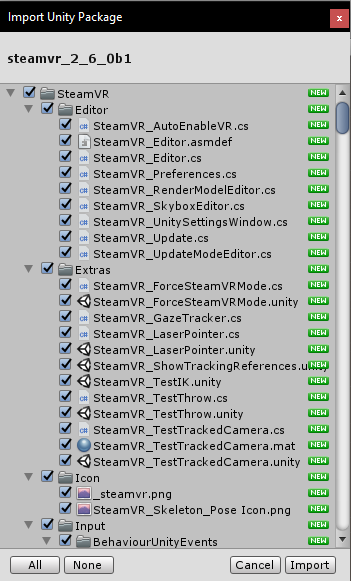
\includegraphics[width=0.5\textwidth]{04.Desarrollo/01.Entrega1/01.Iteracion1_1/00.Figuras/01.steam_vr_import.png}
    \caption{Importación del paquete SteamVR Unity Plugin 2.6.0b1.}
    \label{fig:SteamVRimport}
\end{figure}


Para importar VRTK Prefabs (1.1.11) basta con seguir la documentación disponible en su repositorio de GitHub (\url{https://github.com/ExtendRealityLtd/VRTK.Prefabs}). Solo es necesario modificar el archivo manifest.json del proyecto como se indica en la figura \ref{fig:vrtkPackage}. Este archivo se encarga de gestionar las dependencias de paquetes.

\begin{figure}
  \centering
    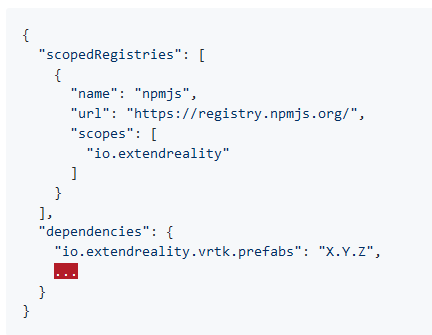
\includegraphics[width=0.7\textwidth]{04.Desarrollo/01.Entrega1/01.Iteracion1_1/00.Figuras/02.vrtk_package.png}
    \caption{Líneas a añadir en manifest.json, siendo X.Y.Z la versión deseada.}
    \label{fig:vrtkPackage}
\end{figure}

Integrar Zinnia (1.16.0) en el proyecto se realiza de la misma forma que VRTK Prefabs, modificando el archivo manifest.json según las instrucciones de su repositorio (https://github.com/ExtendRealityLtd/Zinnia.Unity).

En esta prueba se han utilizado las versiones más recientes de cada uno de los paquetes, pero tras integrar VRTK Prefabs comienzan a aparecer errores de compatibilidad con SteamVR (figura \ref{fig:erroresVrtk}) y resulta imposible continuar.

\begin{figure}
  \centering
    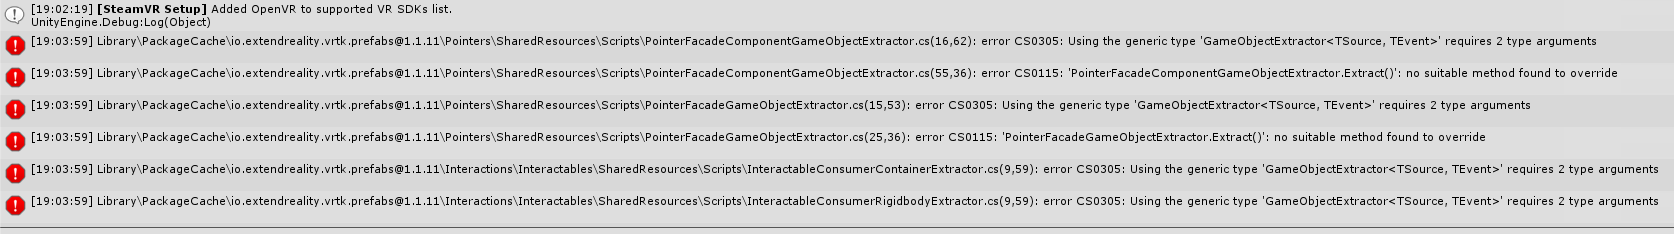
\includegraphics[width=1\textwidth]{04.Desarrollo/01.Entrega1/01.Iteracion1_1/00.Figuras/03.errores_vrtk.png}
    \caption{Errores al importar VRTK Prefabs.}
    \label{fig:erroresVrtk}
\end{figure}

Tras varias pruebas de integración, se han encontrado las versiones de cada paquete que no interfieren entre ellos. Por tanto, en el desarrollo de este proyecto no se van a utilizar las versiones más recientes hasta la fecha de cada uno (mostradas anteriormente), si no que se van a utilizar las siguientes versiones:


\begin{itemize}
	\item{SteamVR Unity Plugin 2.2.0}

	\item{VRTK Prefabs 1.1.5}
	
	\item{Zinnia 1.8.0}

\end{itemize}

Por último, es necesario generar los datos sobre las entradas de SteamVR, para ello se abre la ventana SteamVR Input (figura \ref{fig:inputCompile}) y se pulsa el botón Save and generate.

\begin{figure}
  \centering
    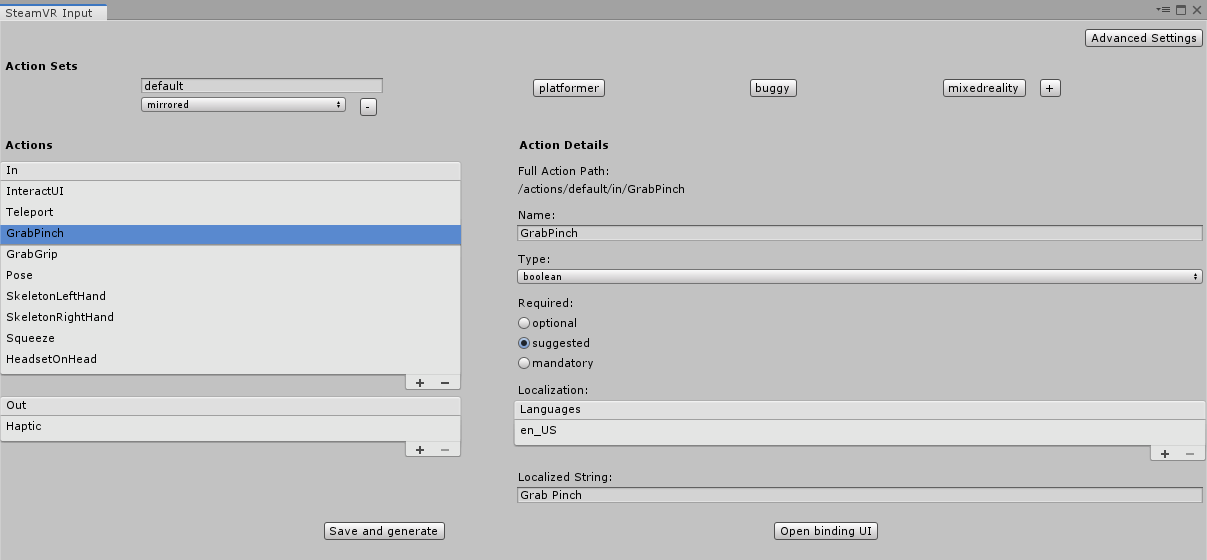
\includegraphics[width=0.8\textwidth]{04.Desarrollo/01.Entrega1/01.Iteracion1_1/00.Figuras/04.input_compile.png}
    \caption{Ventana SteamVR Input.}
    \label{fig:inputCompile}
\end{figure}

Una vez todos los paquetes se han importado de manera correcta, se crea una escena en el proyecto de Unity y en ella se añade un prefab proporcionado por el plugin de SteamVR que contiene todo lo necesario para funcionar con el dispositivo de desarrollo.


